\documentclass{article}

% if you need to pass options to natbib, use, e.g.:
% \PassOptionsToPackage{numbers, compress}{natbib}
% before loading nips_2016
%
% to avoid loading the natbib package, add option nonatbib:
% \usepackage[nonatbib]{nips_2016}

% \usepackage{nips_2016}

% to compile a camera-ready version, add the [final] option, e.g.:
\usepackage[final,nonatbib]{nips_2016}

\usepackage[utf8]{inputenc} % allow utf-8 input
\usepackage[T1]{fontenc}    % use 8-bit T1 fonts
\usepackage{hyperref}       % hyperlinks
\usepackage{url}            % simple URL typesetting
\usepackage{booktabs}       % professional-quality tables
\usepackage{amsfonts}       % blackboard math symbols
\usepackage{nicefrac}       % compact symbols for 1/2, etc.
\usepackage{microtype}      % microtypography
\usepackage{color}
\usepackage{graphicx}
\usepackage{amssymb,amsfonts,amsmath,graphicx}    
\usepackage[shortlabels]{enumerate}
\usepackage[options ]{algorithm2e}
\graphicspath{ {../figures/} }

\newcommand{\ind}[1]{1_{#1}} % Indicator function
\newcommand{\pr}{P} % Generic probability
\newcommand{\ex}{E} % Generic expectation
\newcommand{\var}{\textrm{Var}}
\newcommand{\cov}{\textrm{Cov}}
\newcommand{\sgn}{\textrm{sgn}}
\newcommand{\sign}{\textrm{sign}}
\newcommand{\kl}{\textrm{KL}} 
\newcommand{\abs}[1]{|{#1}|}



\renewcommand{\S}{\Sigma}
\renewcommand{\L}{\Lambda}
\renewcommand{\[}{\begin{equation}}
\renewcommand{\]}{\end{equation}}
\renewcommand{\b}{\backslash}
\newcommand{\g}{\,\vert\,}
\newcommand{\tr}{\mathrm{tr}}
\newcommand{\diag}{\mathrm{diag}}
\newcommand{\bea}{\begin{eqnarray}}
\newcommand{\eea}{\end{eqnarray}}
\newcommand{\hx}{\hat{x}}
\newcommand{\hxi}{\hat{\xi}}
\newcommand{\Var}{\mathrm{Var}}
\newcommand{\Cov}{\mathrm{Cov}}
\newcommand{\prop}{\propto}
\newcommand{\deq}{:=}

\newcommand{\EE}{\mathbb{E}}
\newcommand{\II}{\mathbb{I}}
\newcommand{\R}{\mathbb{R}}
\newcommand{\PP}{\mathbb{P}}

\newcommand{\La}{\mathcal{L}}

\newcommand{\n}{\mathcal{N}}

\newcommand{\bx}{\mathbf{x}}
\newcommand{\bX}{\mathbf{X}}
\newcommand{\by}{\mathbf{y}}
\newcommand{\bs}{\mathbf{s}}
\newcommand{\bn}{\mathbf{n}}
\newcommand{\br}{\mathbf{r}}
\newcommand{\bt}{\mathbf{t}}

\newcommand{\fig}[1]{Figure~\ref{fig:#1}}
\newcommand{\chap}[1]{Chapter~\ref{chap:#1}}
\newcommand{\mysec}[1]{Section~\ref{sec:#1}}
\newcommand{\app}[1]{Appendix~\ref{sec:#1}}
\newcommand{\eq}[1]{Eq.~(\ref{eq:#1})}
\newcommand{\eqs}[1]{Eqs.~(\ref{eq:#1})}
\newcommand{\eqss}[1]{(\ref{eq:#1})}
\newcommand{\thm}[1]{Theorem~\ref{thm:#1}}

\newcommand{\indep}{{\;\bot\!\!\!\!\!\!\bot\;}}
\newcommand{\eps}{\varepsilon}

\newcommand{\one}{1}
\newcommand{\Dir}{{\rm Dir}}
\newcommand{\Mult}{{\rm Mult}}
\newcommand{\Bin}{{\rm Bin}}
\newcommand{\Ga}{{\rm Ga}}
\newcommand{\IG}{{\rm IG}}
\newcommand{\InvGa}{{\rm IG}}
\newcommand{\Chisquare}{\Chi^2}
\newcommand{\St}{{\rm St}}
\newcommand{\Beta}{{\rm Beta}}
\newcommand{\iid}{i.i.d.}
\newcommand{\Eta}{{\cal N}}
\newcommand{\Ber}{{\rm Ber}}

\newcommand{\simiid}{\stackrel{\tiny\text{iid}}{\sim}}
\newcommand{\simind}{\stackrel{\tiny\text{ind}}{\sim}}

\DeclareMathOperator*{\BP}{BP}
\DeclareMathOperator*{\DP}{DP}
\DeclareMathOperator*{\GP}{GP}
\DeclareMathOperator*{\BeP}{BeP}

% Caligraphic alphabet
\newcommand{\calr}{\mathcal{R}} % only because \cr already taken
\newcommand{\ca}{\mathcal{A}} \newcommand{\cb}{\mathcal{B}} \newcommand{\cc}{\mathcal{C}} \newcommand{\cd}{\mathcal{D}} \newcommand{\ce}{\mathcal{E}} \newcommand{\cf}{\mathcal{F}} \newcommand{\cg}{\mathcal{G}} \newcommand{\ch}{\mathcal{H}} \newcommand{\ci}{\mathcal{I}} \newcommand{\cj}{\mathcal{J}} \newcommand{\ck}{\mathcal{K}} \newcommand{\cl}{\mathcal{L}} \newcommand{\cm}{\mathcal{M}} \newcommand{\cn}{\mathcal{N}} \newcommand{\co}{\mathcal{O}} \newcommand{\cp}{\mathcal{P}} \newcommand{\cq}{\mathcal{Q}} \newcommand{\cs}{\mathcal{S}} \newcommand{\ct}{\mathcal{T}} \newcommand{\cu}{\mathcal{U}} \newcommand{\cv}{\mathcal{V}} \newcommand{\cw}{\mathcal{W}} \newcommand{\cx}{\mathcal{X}} \newcommand{\cy}{\mathcal{Y}} \newcommand{\cz}{\mathcal{Z}}

% Convergence
\newcommand{\convd}{\stackrel{d}{\longrightarrow}} % convergence in distribution/law/measure
\newcommand{\convp}{\stackrel{P}{\longrightarrow}} % convergence in probability
\newcommand{\convas}{\stackrel{\textrm{a.s.}}{\longrightarrow}} % convergence almost surely
\newcommand{\convr}{\stackrel{r}{\longrightarrow}} % convergence in r^{th} mean

\newcommand{\eqd}{\stackrel{d}{=}} % equal in distribution/law/measure
\newcommand{\argmax}{\mathop{\mathrm{argmax}}}
\newcommand{\argmin}{\mathop{\mathrm{argmin}}}
\newcommand{\conv}{\textrm{conv}} % for denoting the convex hull


\makeatletter
\providecommand*{\diff}%
	{\@ifnextchar^{\DIfF}{\DIfF^{}}}
\def\DIfF^#1{%
	\mathop{\mathrm{\mathstrut d}}%
		\nolimits^{#1}\gobblespace}
\def\gobblespace{%
	\futurelet\diffarg\opspace}
\def\opspace{%
	\let\DiffSpace\!%
	\ifx\diffarg(%
		\let\DiffSpace\relax
	\else
		\ifx\diffarg[%
			\let\DiffSpace\relax
	\else
		\ifx\diffarg\{%
			\let\DiffSpace\relax
		\fi\fi\fi\DiffSpace}


\providecommand*{\deriv}[3][]{\frac{\diff^{#1}#2}{\diff #3^{#1}}}
\providecommand*{\pderiv}[3][]{\frac{\partial^{#1}#2}{\partial #3^{#1}}}
		
\newcommand{\threequals}{\equiv}

\usepackage{subcaption}


\title{Data Augmentation to Accelerate Convergence of Variational Bayes}

% The \author macro works with any number of authors. There are two
% commands used to separate the names and addresses of multiple
% authors: \And and \AND.
%
% Using \And between authors leaves it to LaTeX to determine where to
% break the lines. Using \AND forces a line break at that point. So,
% if LaTeX puts 3 of 4 authors names on the first line, and the last
% on the second line, try using \AND instead of \And before the third
% author name.

\author{
  Runjing Liu and Jake Soloff \\
  Department of Statistics, UC Berkeley\\
  \texttt{\{runjing\_liu,jake\_soloff\}@berkeley.edu}
  %% examples of more authors
  %% \texttt{email} \\
  %% \And
  %% Coauthor \\
  %% Affiliation \\
  %% Address \\
  %% \texttt{email} \\
  %% \And
  %% Coauthor \\
  %% Affiliation \\
  %% Address \\
  %% \texttt{email} \\
}

\begin{document}
% \nipsfinalcopy is no longer used

\maketitle

\vspace{-1em}

\begin{abstract}
one line\\two lines\\3 linez\\ 4 linsu
\end{abstract}

\section{Motivation}
\label{motivation}
%Voting records of legislators are commonly analyzed by political scientists to examine relationships between legislator political leanings, institutional structures, and legislative outcomes \cite{Clinton2004}. For example, even simple dimensionality reduction techniques on voting data in the US House of Representatives uncover the political characteristics of individual legislators such as party affiliation (Figure \ref{fig:DimRedux}). \par

\subsection{Optimization as Approximate Inference} 

Bayesian statistics offers a simple formula for learning from data: specify a joint distribution $p(X,\theta) = p(X\mid \theta)\,p(\theta)$ over observations $X$ and latent variables $\theta$, and quantify the uncertainty in $\theta$ conditional on seeing $X$ through the posterior distribution $p(\theta\mid X)$. In complex models, exact computation with the full posterior is intractable \cite{Cooper}; in practice, we turn to methods for approximation such as sampling (MCMC) or variational inference.

{\sl Variational Bayes} casts posterior inference as an optimization problem
\begin{align}
\min_{q}D(q(\theta)\,\|\, p(\theta\mid X)).
\end{align}
Since the KL-divergence is non-negative and vanishes precisely at $q(\theta) = p(\theta\mid X)$, this program recovers the target. We focus on variational Bayes under the na\"ive mean field assumption, which restricts the minimization in equation (1) to all distributions $q(\theta) = \prod_{i=1}^Kq(\theta_i)$ which factorize over the latent variables $\theta = \{\theta_i\}_{i=1}^K$. Noting that
\begin{align}
\mathcal L(q) :=  \mathbb E_q\left[\log\frac{p(X,\theta)}{q(\theta)}\right] =\log p(X) -  D(q(\theta)\,\|\, p(\theta\mid X)) \le \log p(X).
\end{align}
The quantity $\mathcal L(q)$ (called the ELBO) lower bounds the model evidence, and the program (1) is equivalent to maximizing $\mathcal L(q)$. We may impose parametric assumptions on each variational factor $q(\theta_i) = q_{\widehat\tau_i}(\theta_i)$ to simplify the expectations in equation (2) and optimize over the choice of $\widehat\tau_i$---though we emphasize that in many cases these additional assumptions are unnecessary \cite{Beal,Blei}. Coordinate ascent variational inference (CAVI) maximizes $\mathcal L(q)$ over each factor individually with the others held fixed. 

Note that CAVI does not recover the true posterior, in contrast with Gibbs sampling, which is {\sl asymptotically} exact. Compared to sampling, however, Variational Bayes tends to be more efficient, as we can leverage many tools from optimization. Both methods are known to converge slowly when the latent variables are well correlated in the posterior. In the appendix, we show this for a Gaussian posterior, where the rates for the Gibbs sampler (as computed in \cite{Sahu}) and CAVI actually match:

{\bf Proposition 1.} Consider a model in which the posterior distribution has form
\begin{align}
p(\theta\mid X) \triangleq \mathcal N(\mu^*,\Lambda^{-1}),
\end{align}
where $\mu^* = (\mu_1^*,\mu_2^*)^{\mathsf T}$ and $\Lambda$ has blocks $\Lambda_{11}, \Lambda_{12},$ and $\Lambda_{22}$, and these means and precisions depend implicitly on the observation $X$. Then CAVI, which updates blocks $\theta_1$ and $\theta_2$ alternatingly, converges linearly at the same rate as the corresponding Gibbs sampler.

\newpage

\subsection{Reparametrization for Accelerated Convergence} 

\subsection{Example: Normal Hierarchical Model} 

\newpage

\section{Parameter Expanded Variational Bayes}
\label{PXVB}

We describe here the Parameter Expanded Variational Bayes (PX-VB) algorithm proposed in \cite{Qi2006}. Suppose we have a data model $p(X,\theta)$, where $\theta =  \{\theta_1, ... , \theta_K\}$ are parameters, and $X$ represents the observed data. In PX-VB, the data model is augmented with an auxiliary parameter $\alpha$. Denote this overparametrized model by $p_\alpha(\theta, X)$; and let $\alpha_0$ be the choice of $\alpha$ where the original model is recovered. PX-VB adds two additional steps to the standard CAVI algorithm. At every iteration, we run one step of CAVI, which outputs an approximate variational distribution. PX-VB then chooses an $\alpha$ with which we will expand the data model. The original objective is then recovered through reparametrization of the variational distribution. In other words, any changes incurred by adjusting the data model from $\alpha_0$ to $\alpha$ is absorbed into the variational distribution $q(\theta)$. 



More precisely, at the $t$-th iteration, PX-VB does the following: 
\begin{enumerate}[(i)]
\item {\bf Coordinate ascent:} Sequentially update $q^{(t)}(\theta_i)$, for $i=1,..., K$ to minimize $D\big( \prod_{i=1}^K q(\theta_i) \| p_{\alpha_0}(\theta, X) \big)$. 
\item {\bf Expand:} Choose $\alpha$ to minimize $D\big( \prod_{i=1}^K q^{(t)}(\theta_i) \| p_\alpha(\theta, X) \big)$.
\item {\bf Reduce:} Choose a reparametrization $\theta \mapsto \hat\theta$ such that
\begin{align*}
D\Big( \prod_{i=1}^K q^{(t)}(\hat\theta_i) \,\big\|\, p_{0}(\hat\theta, X) \Big) = D\Big( \prod_{i=1}^K q^{(t)}(\theta_i) \,\big\|\, p_\alpha(\theta, X) \Big)
\end{align*}
Set $q^{(t+1)}(\theta) = q^{(t)}(\hat\theta)$, and repeat. 
\end{enumerate}


Note that with these two added steps to CAVI, PX-VB remains a descent algorithm. In step 2, our choice of $\alpha$ ensures that the KL decreases, and in step three, we reparametrize $q^{(t)}(x)$ to maintain this KL. Therefore, one iteration of PX-VB should do no worse than one step of CAVI on its own. 

The added steps of PX-VB increase the computational cost compared to CAVI, but with a proper choice of augmentation,  PX-VB often converges in fewer iterations, as we explore in the sequel. We see two explanations for such behavior. Firstly, the reparametrization allows for exploration of the parameter space in directions other than the coordinate axes. In the extreme case of the normal hierarchical model, PX-VB points the trajectory of the updates directly to the correct posterior means. Secondly, running CAVI to find an optimal mean field approximation suffers from slow convergence when the variables in the factorized distribution are strongly correlated. A good reparametrization in PX-VB helps decouple the these variables to achieve faster convergence. 




\section{Example: Probit Regression}
\label{probit}

Following the example in \cite{Qi}, we explore the performance of PX-VB in the setting of Bayesian probit regression. Let $\{t_n\}_{n=1}^N$ be $\{-1,+1\}$--valued random variables. The design matrix $X\in\mathbb R^{N\times D}$ is fixed, and we place a normal prior on the parameter vector $w\in\mathbb R^D$. The generative model is
\begin{align}
w &\sim \mathcal N (0, v_0^2) \\
t_n &\sim \text{Bern}(\Phi(w^\mathsf T x_n))\quad \text{n = 1, ..., N} \label{eq:gen_probit_1}
\end{align}
where $\Phi$ is the standard normal c.d.f. Equivalently, we can re-write this generative model with latent variables $z_n$ as follows: 
\begin{align}
    w &\sim \mathcal N (0, v_0^2) \\
    z_n &\sim \mathcal N (w^\mathsf T x_n, 1)\quad \text{n = 1, ..., N} \label{eq:gen_probit_zn}\\
    t_n &= \text{sign}(z_n) \quad \text{n = 1, ..., N} \label{eq:gen_probit_2}
\end{align}
A brief computation verifies this equivalence: 
\begin{align}
P(t_n = +1) &= P(z_n \geq 0) \quad \text{(by eqn. \ref{eq:gen_probit_2} )}\\
&= \Phi(w^\mathsf Tx_n) \quad \text{(by eqn. \ref{eq:gen_probit_zn})}
\end{align}
which shows that $t_n$ is Bernoulli with parameter $\Phi(w^\mathsf Tx_n)$. 

\subsection{Parameter updates}
We will work with the second formulation with the latent $z_n$. We take a fully factorized distribution over $\{z_n\}_{n=1}^N$ and $w$. In particular, 
\begin{align}
    q_w(w) &\sim \mathcal N (\hat w, \hat\Sigma_w)\\
    q_{z_n}(z_n) &\sim \mathcal{N}(\hat z_n, 1)\mathbb I\{\text{sign}(z_n) = t_n\}
\end{align}
That is, $q_{z_n}$ follows a truncated normal distribution; $z_n$ is restricted to $[0,\infty)$ or $(-\infty,  0]$ when $t_n=1$ or $t_n=-1$, respectively. Our goal is to find parameters $\{z_n\}_{n=1}^\infty$, $\hat w$, and $\hat\Sigma_w$ to minimize the KL divergence $D\big(q(w) \prod_{n=1}^N q(z_n)\|p(w, z| t)\big)$, where $p(w,z|t)$ is the true posterior distribution. 

Writing out this objective explicitly (see \ref{probit_append}) we find that the coordinate ascent updates for the variational parameters are given by 
\begin{align}
    \hat z_n &= \hat w^T x_n \quad n = 1, ..., N\\
    \Sigma_w &= (X^T X + v_0^{-2} I_{D\times d})^{-1}\\
    \hat w &= (X^T X + v_0^{-2} I_{D\times d})^{-1} XE_q[z]
\end{align}

Now we seek to use PX-VB to accelerate the convergence of CAVI. We augment our model as follows with an auxiliary parameter $\alpha$ as follows: 
\begin{align}
    w &\sim \mathcal N (0, \alpha v_0^2) \\
    z_n &\sim \mathcal N (w^\mathsf T x_n, \alpha)\quad \text{n = 1, ..., N} \label{eq:gen_probit_zn}\\
    t_n &= \text{sign}(z_n) \quad \text{n = 1, ..., N} \label{eq:gen_probit_2}
\end{align}
In other words, we expanded the original model $p(w,z,t|X)$ to $p_\alpha(w,z,t|X)$ with the relation
\begin{align}
   p_\alpha(w,z,t|X) = p(\alpha w, \alpha z, t|X)
\end{align}

In step (ii) of PX-VB, we minimize $D\big(q(w) \prod_{n=1}^N q^{(t)}(z_n) \| p_\alpha(w,z,t|X) \big)$ with respect to $\alpha$ and find that (see \ref{probit_append}
\begin{align}
    \alpha^{*2} = \frac{1}{N+M} \Big(\sum_{n=1}^N E_q[z_n^2] - 2E_q[z_n] \hat w^\mathsf Tx_n + x_n^\mathsf T E_q[w w^\mathsf T] w_n\Big) + \frac{1}{v_0^2(N+M)} E_q[w w^\mathsf T]
\end{align}

And in step (iii) the original model is recovered by taking
\begin{align}
    q^{(t+1)}(w) = q^{(t)}(w/\alpha^*) \quad \text{and} \quad q^{(t+1)}(z_n) = q^{(t)}(z_n/\alpha^*)
\end{align}
Note that the added steps in PX-VB are relatively computationally inexpensive, and in the following sections, we explore the gains in the rate of convergence. 

\subsection{Simulated Data}
We compare the convergence of three algorithms: CAVI, PX-VB, and Newton conjugate gradient trust region. First, we applied these algorithms on simulated data: we took the number of data points $N = 500$, the dimension of the parameter $w$ was 20. The results are displayed in figure~\ref{fig:Probit_synth}. 



\begin{figure}[h]
        \begin{subfigure}[t]{0.49\textwidth}
        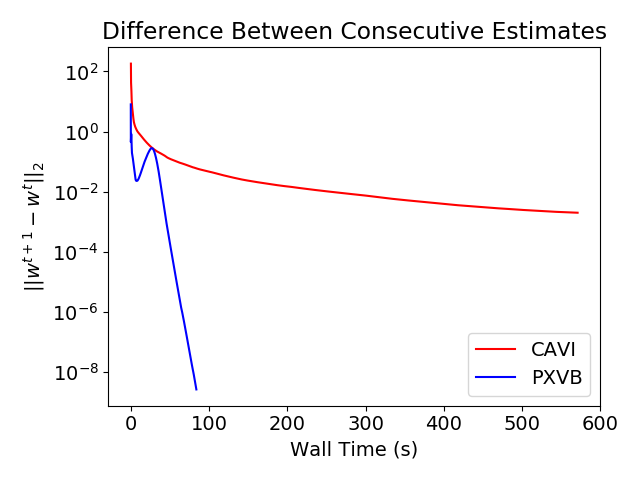
\includegraphics[width=\textwidth]{Probit_real/CAVI_PX_convergence.png}
    \end{subfigure}
          \begin{subfigure}[t]{0.49\textwidth}
        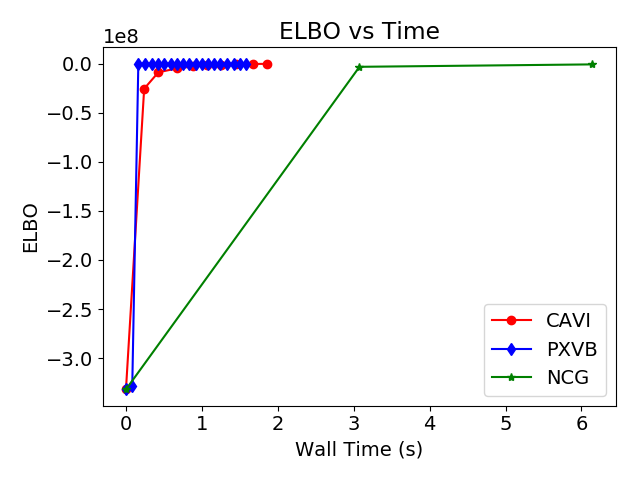
\includegraphics[width=\textwidth]{Probit_real/elbo_time.png}
    \end{subfigure}
    \caption{Convergence results for variational inference on SPAM dataset [2], consisting of $N= 4601$ emails, each with $D=57$ keyword predictors (see examples in table). The response variables $t_n$ indicate whether the email was spam.} %The consecutive differences in the second order method did not exhibit as much regularity, so they are omitted on the first plot.}
    \label{fig: Probit_synth}
\end{figure}



\subsection{SPAM Data}



\begin{figure}[h]
        \begin{subfigure}[t]{0.49\textwidth}
        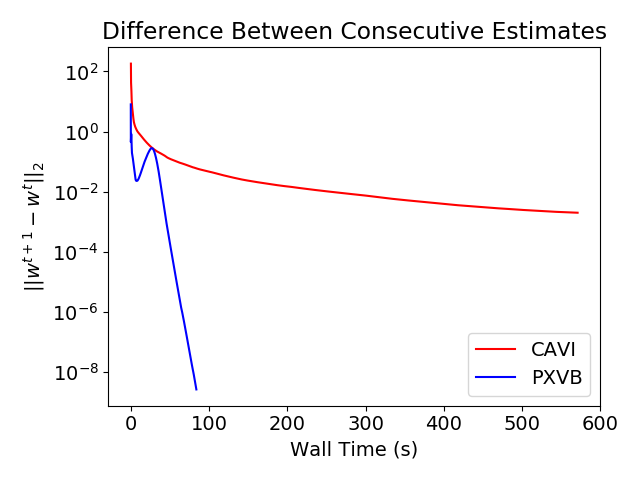
\includegraphics[width=\textwidth]{Probit_real/CAVI_PX_convergence.png}
    \end{subfigure}
          \begin{subfigure}[t]{0.49\textwidth}
        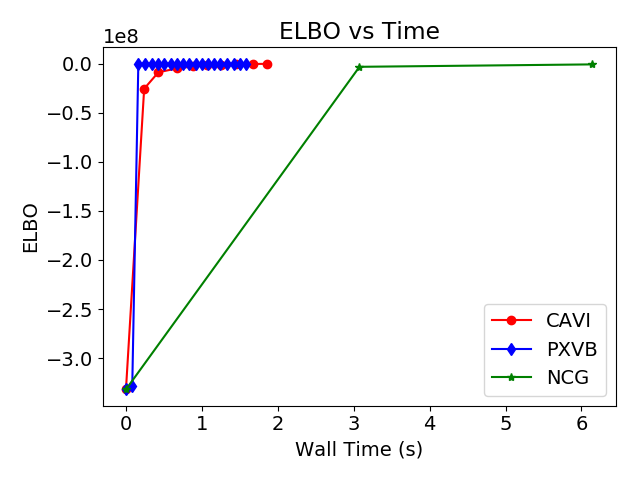
\includegraphics[width=\textwidth]{Probit_real/elbo_time.png}
    \end{subfigure}
    \caption{Convergence results for variational inference on SPAM dataset [2], consisting of $N= 4601$ emails, each with $D=57$ keyword predictors (see examples in table). The response variables $t_n$ indicate whether the email was spam.} %The consecutive differences in the second order method did not exhibit as much regularity, so they are omitted on the first plot.}
    \label{fig: Probit_spam}
\end{figure}

\section{Example: Linear Mixed Models} 
As in the Probit model, let $X\in \mathbb{R}^{N\times D}$ be a fixed design matrix, with rows $x_n, n = 1,..., N$. We also assume the variances $\sigma^2_\beta, \sigma^2_\mu$, and $\sigma^2_y$ are fixed and known. Let the number of groups be $N_G$, and let the mapping $g(n)\mapsto \{1, ..., N_G\}$ denote the group to which the $n$-th individual belongs. Then the linear mixed model is formulated is follows: 
\begin{align}
\beta &\sim \mathcal N(0, \sigma^2_\beta I_{D\times D})\\
\mu_g &\sim \mathcal N(0, \sigma^2_\mu) \quad \text{for $g= 1, ..., N_G$} \\
y_n | \mu_g, \beta &\sim \mathcal N (x_n^T\beta + \mu_{g(n)}, \sigma^2_y)\quad \text{for $n = 1, ..., N$}
\end{align}
We take a fully factorized distribution over $\beta$ and $\{\mu_g\}_{g=1}^{N_G}$. In particular, 
\begin{align}
q_\beta(\beta) &\sim \mathcal N (\hat \beta, \Sigma_\beta)\\
q_{\mu_g}(\mu_g) &\sim \mathcal{N}(\hat\mu_g, \tau^2_{\mu_g}) \quad \text{for }g = 1, ..., N_G
\end{align}
The updates for the variational parameters $\hat\beta$, $\Sigma_\beta$, $\hat\mu_g$, and $\tau^2_{\mu_g}$ are standard exponential family computations. They are given by 
\begin{align}
{\tau^2_{\mu_g}} &= \Big(\frac{1}{\sigma^2_\mu} + \frac{|\{n : g(n) = g\}|}{\sigma^2_y}\Big)^{-1}\\
{\hat\mu_g} &= \Big(\frac{1}{\sigma^2_\mu} + \frac{|\{n : g(n) = g\}|}{\sigma^2_y}\Big)^{-1}\Big(\frac{1}{\sigma^2_y}\sum_{n: g(n) = g} (y_n - x_n^T\hat\beta)\Big)
\end{align}
for $g = 1, ..., N_G$. and 
\begin{align}
\Sigma_\beta &= (\frac{1}{\sigma^2_\beta} + \frac{1}{\sigma^2_y}XX^T)^{-1}\\
\hat\beta &= (\frac{1}{\sigma^2_\beta} + \frac{1}{\sigma^2_y}XX^T)^{-1}\Big(\frac{1}{\sigma^2_y}\sum_{n=1}^N  x_n(y_n - \hat\mu_{g(n)} )\Big)
\end{align}




\section{Discussion}
We found that in our Bayesian probit regression problem, PX-VB speeds up the convergence of variational methods compared to coordinate ascent and Newton conjugate gradient, two standard algorithms in optimization. The advantage to a Newton method is that there exist "black box" implementations of such algorithms in most standard optimization packages. The only requirement is that one must be able to write down the objective function, in our case the evidence lower bound. However, in variational methods, the optimization is often conducted over a high dimensional parameter space. For example, in the linear mixed model, there is at least one variational parameter for each group, and in the probit regression, there are at least one for each data point. This results in high computational complexity at each iteration. This phenomenon is well exhibited in our results, where Newton suffers in terms of wall time, even though the number of iterations required for convergence may often be much smaller than CAVI or PX-VB. 

Thus, our result suggest that there are real gains in convergence time to deriving updates for coordinate descent. While CAVI requires more iterations to converge than Newton, each iteration is very cheap to compute. 


PX-VB introduces an intermediate step to coordinate ascent, but the computational cost of this additional step is often small---and with a good augmentation, this additional computational cost is made worthwhile by the gains in per-iteration rate of convergence as demonstrated in the Probit model.

To see this more abstractly, we can view the intermediate step in PX-VB as defining a mapping $M$ that takes $(q, p_0) \stackrel{\text{(ii)}}{\mapsto} (q, p_\alpha) \stackrel{\text{(iii)}}{\mapsto} (q_\alpha, p_0)$. Moreover, let $S$ be the mapping defined by the CAVI updates, and assume that the truth $q^*$ is a fixed point of both the mappping $S$ and $M$. Then the error of each iteration of PX-VB can be seen as
\begin{align}
\|q^{(t+1)} - q^*\|_2 &\leq \| M(S(q^{(t)})) - q^*\|_2 \\
&\leq \|MS\|_2 \|q^{(t)} - q^*\|_2\\
&\leq \|M\|_2\|S\|_2 \|q^{(t)} - q^*\|_2
\end{align}

Thus, we see that while CAVI converges linearly at rate $\|S\|_2$, PX-VB converges at rate $\|M\|_2\|S\|_2$. Whenever the largest eigenvalue of $M$ is less than $1$, PX-VB will converge faster than CAVI. 

{\color{red} depending on how LMM turns out, put more on LMM here. Was our $M$ bad for LMM} 




\section{Conclusions and future directions} 
One challenge to running PX-VB is anticipating which data-augmentation scheme will actually accelerate convergence. 

It is well known that the mean field approximation performs well when the posterior distribution has low correlation. Therefore, we would like to understand the connection between the reparametrization mapping $M$ and the posterior correlation structure. ~\\~\\

Ultimately, in the normal hierarchical model, data augmentation methods correspond to choosing good directions for coordinate ascent. We would like to look at more examples where PX-VB succeeds and understand whether, more generally, these directions make use of second-order structure.


\newpage

\section*{Acknowledgments}
We would like to thank Professor Wainwright and Fanny for their dedication to teaching an excellent course! % also thank ryan %Also thanks to the stat department lounge for housing us since we got here.

\section*{Attribution}
\begin{itemize}
\item Runjing Liu: 
\item Jake Soloff: 
\end{itemize}

\begin{thebibliography}{10}

\bibitem{Beal} Beal, M. (2003). Variational Algorithms for Approximate Bayesian Inference. {\sl Doctoral dissertation}, Gatsby Computational Neuroscience Unit, University College London.

\bibitem{Blei} Blei, D. M., Kucukelbir, A. \& McAuliffe, J. D. (2016). Variational Inference: a Review for Statisticians. {\itshape arXiv:1601.00670}.

\bibitem{Cooper} Cooper, G.F. (1990). The Computational Complexity of Probabilistic Inference using Bayesian Belief Networks. {\sl Artificial Intelligence.} 42(2), 393–405.

\bibitem{Efron} Efron, B \& Hastie, T.J. (2016). Computer Age Statistical Inference. {\itshape Cambridge University Press}.

\bibitem{Grimmer} Grimmer, J. (2011). An Introduction to Bayesian Inference via Variational Approximations. {\itshape Political Analysis}. 19(1): 32-47.

\bibitem{Luo} Luo, Z. Q. \& Tseng, P. (1992). On the Convergence of the Coordinate Descent Method for Convex Differentiable Minimization. {\itshape Journal of Optimization Theory and Applications} 72(1): 7-35. 

\bibitem{Qi} Qi, Y. \& Jaakkola, T. S. (2006). Parameter Expanded Variational Bayesian Methods. {\itshape Neural Information Processing Systems}. 

\bibitem{Sahu} Sahu, S. K., and Roberts, G. O. (1998), On Convergence of the EM Algorithm and the Gibbs Sampler. {\sl Statistics
and Computing}. 

\bibitem{Yu} Yu, Y. \& Meng, X. (2012). To Center or Not to Center: That Is Not the
Question-- An Ancillarity-Sufficiency Interweaving Strategy (ASIS) for Boosting MCMC Efficiency. {\itshape Journal of Computational and Graphical Statistics}. 20(3): 531-570. 
\end{thebibliography}

\newpage

\appendix

\section{Variational updates}
\label{vi}
\subsection{Probit Model}
\label{probit_append}

\noindent{\bf Variational Factors.} 

\noindent{\bf Computing the ELBO.} Now we can write out the component terms of the ELBO more explicitly:

\noindent{\bf CAVI Updates.} 
%The simplest approach to variational inference maximizes the ELBO $\cl$ via coordinate-ascent, i.e. choosing the best value of a variational parameter with all others fixed. Iteratively applying these updates, the variational approximation $q$ improves at every step toward some local optimum. Conditional conjugacy yields closed form updates for $\widehat\gamma_k$ and $\widehat\lambda_{kl}$:

\begin{itemize}
\item {\bf Update to $q(\pi)$.} 
\item {\bf Update to } 
\item {\bf Update to }
\end{itemize}


\subsection{Linear Mixed Model}
\label{lmm}


\subsection{Normal Means Model}
\label{normal}








\end{document}